\section{问题四：观测收缩下的干燥过程}
\label{sec:q4}

\begingroup
% Local display spacing accommodates the introduction; text and figure sizes are unchanged.
\setlength{\abovedisplayskip}{8pt plus 2pt minus 2pt}
\setlength{\belowdisplayskip}{8pt plus 2pt minus 2pt}
\setlength{\abovedisplayshortskip}{6pt plus 2pt minus 1pt}
\setlength{\belowdisplayshortskip}{6pt plus 2pt minus 1pt}
问题四在第\ref{sec:common-model}章统一模型基础上，结合附件2的观测半径，
在恒长度、均匀径向收缩假设下，用材料坐标与干物质守恒处理几何变化。
采用附录4物性，从共同初态联立求解温湿场，沿用问题三的径向最大含水率判据
确定所设环境条件下的模型干燥时长，并通过同物性恒半径对照分析收缩作用。
求解流程见图\ref{fig:q4-workflow}。

\begingroup
\setlength{\intextsep}{10pt}
\begin{figure}[H]
\centering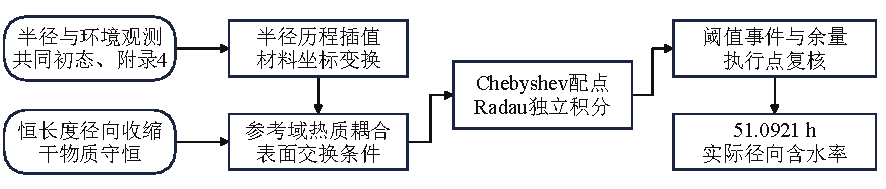
\includegraphics[width=\linewidth]{figures/legibility_schematics/q4_workflow.pdf}
\caption{问题四的收缩模型求解流程}
\label{fig:q4-workflow}
\end{figure}
\endgroup

\subsection{半径历程与材料运动}

问题四将附录4物性代入式\eqref{eq:heat}--\eqref{eq:boundary}，
并根据附件2把固定几何改为运动材料域。
温度和含水率从28\celsius、2.55\unit{kg/kg}的共同初态重新求解，
不接续问题三的干燥末态。
附件2含0--72\unit{h}的145个半径记录，间隔1800\unit{s}，
半径由2\unit{cm}降至1.198\unit{cm}。
本文将半径转换为米后分段线性插值为$R(t)$，
保持其单调性和平台段；所求主终点位于观测时域内。
环境继续采用前4\unit{h}观测插值及之后的共同均值平台。

外半径只规定边界位置，不能唯一确定内部材料运动。
采用均匀径向收缩、长度$L=L_0$不变的运动学闭合，
定义材料标记$\xi$及映射
\begin{equation}
 r=R(t)\xi,\quad z=Z,\qquad
 v_{s,r}=\frac{R'(t)}{R(t)}r=w_r,\quad v_{s,z}=0,
 \qquad J=\left(\frac{R(t)}{R_0}\right)^2.
 \label{eq:radius-map}
\end{equation}
其中$w_r=\partial r/\partial t|_\xi$为网格速度，$J$为体积Jacobian。
该材料映射是一项附加假设，而不是半径记录直接测得的内部变形。
移动边界模型须区分体积水浓度与材料干基含水率，
并以当前界面的相对通量写守恒条件\cite{adrover2020}。

\subsection{干基守恒与参考域方程}

当前体积水浓度为$\rho_d C$。
对干物质与水分别写守恒式，并采用相对材料的扩散通量，得
\begin{equation}
 \begin{aligned}
  &\partial_t\rho_d+\nabla\cdot(\rho_d\boldsymbol v_s)=0,\\
  &\partial_t(\rho_d C)
   +\nabla\cdot(\rho_d C\boldsymbol v_s+\boldsymbol j_w)=0,
  \qquad \boldsymbol j_w=-\rho_dD\nabla C.
 \end{aligned}
 \label{eq:q4-component-balance}
\end{equation}
第二式减去第一式的$C$倍，即得到式\eqref{eq:moisture}。
由初始干密度均匀和式\eqref{eq:radius-map}，
$\rho_d J=\rho_{d,0}$，所以
$\rho_d(t)=\rho_{d,0}[R_0/R(t)]^2$为空间常数，可从干基水分方程中约去。
对任一场量$f(r,t)=\widehat f(\xi,t)$，链式法则给出
\begin{equation}
 \left.\partial_t f\right|_r
 =\left.\partial_t\widehat f\right|_\xi
   -\frac{R'}R\xi\partial_\xi\widehat f,
 \qquad
 v_{s,r}\partial_r f=\frac{R'}R\xi\partial_\xi\widehat f.
 \label{eq:q4-chain-rule}
\end{equation}
两项中的材料运动恰好抵消，故$\Ds f/\dd t=\partial_t\widehat f|_\xi$。
再将$\partial_r=R^{-1}\partial_\xi$代入式\eqref{eq:heat}和\eqref{eq:moisture}，
省略场量帽号后，一维参考域方程为
\begin{equation}
 \begin{aligned}
  \left.\partial_t C\right|_\xi
   &=\frac{1}{R(t)^2\xi}\partial_\xi
     \left[\xi D(T,C)\partial_\xi C\right],\\
  \rho_{\mathrm{eff}}(C)c_p(C)
   \left.\partial_t T\right|_\xi
   &=\frac{1}{R(t)^2\xi}\partial_\xi
     \left[\xi k(C)\partial_\xi T\right].
 \end{aligned}
 \label{eq:q4-reference-pde}
\end{equation}
轴线取正则对称条件；将同一空间导数变换代入式\eqref{eq:boundary}，
当前侧表面的边界式为
\begin{equation}
 -\frac{D(T_s,C_s)}{R}\left.\partial_\xi C\right|_1=h_m(C_s-b),
 \qquad
 -\frac{k_s}{R}\left.\partial_\xi T\right|_1=h_T(T_s-T_a).
 \label{eq:q4-reference-boundary}
\end{equation}
其中$k_s=k(C_s)$，表面系数均按当前温湿状态计算。

式\eqref{eq:q4-reference-pde}没有额外的几何浓缩源。
无交换的纯收缩使体积水浓度$\rho_d C$增加，
但水与干物质质量均不变，因此干基$C$应保持不变。
若再加入$-2R'C/R$或另一个网格对流项，就会重复计算已经包含的材料运动。
附录$\rho_{\mathrm{eff}}$用于有效热容量，$\rho_d$用于上述质量账本；
二者不能同时通过$\rho_d=\rho_{\mathrm{eff}}/(1+C)$强制等同为真实组分密度。
热式仍无显式潜热，数值闭合不构成真实组分总焓守恒的证明（见第\ref{sec:limitations}节）。

附录4的局部扩散系数为
\begin{equation}
 D(T,C)=4.2\times10^{-4}
 \exp(-0.30/C)
 \exp\!\left[-\frac{3850}{T+273.15}\right].
 \label{eq:q4-diffusivity}
\end{equation}
全部热物性也在各空间位置按当前$C$更新，
温湿两场继续联立求解。
表面交换系数沿用$h_T=25\unit{W/(m^2\cdot K)}$、
$h_m=8\times10^{-7}\unit{m/s}$，
式\eqref{eq:q4-reference-boundary}中的质量通量相对于材料界面，
不另将表面扫过的体积计为蒸发失水。

\subsection{数值求解、账本与结束状态}

令$x=\xi^2$，对任意扩散系数$a$和场量$f$有
\begin{equation}
 \frac{1}{R^2\xi}\partial_\xi(a\xi\partial_\xi f)
 =\frac4{R^2}\partial_x(ax\partial_x f)
 =\frac4{R^2}\bigl[q+x\partial_xq\bigr],
 \qquad q=a\partial_xf.
 \label{eq:q4-x-operator}
\end{equation}
该式消去轴线显式奇点，在$x=0$处直接取$4q(0)/R^2$。
依式\eqref{eq:primitive}定义$F_4'(C)=\exp(-0.30/C)$、$F_4(0)=0$，
并令$A_4(T)=4.2\times10^{-4}\exp[-3850/(T+273.15)]$。
沿用问题二的Chebyshev微分矩阵$\mathsf D_x$，
记$q_{T,i}=k(C_i)(\mathsf D_x\boldsymbol T)_i$、
$q_{C,i}=A_4(T_i)[\mathsf D_x F_4(\boldsymbol C)]_i$
及$S_i=\rho_{\mathrm{eff}}(C_i)c_p(C_i)$，则内部节点方程为
\begin{equation}
 \begin{aligned}
  \dot T_i&=\frac4{R(t)^2S_i}
       \bigl[q_{T,i}+x_i(\mathsf D_x\boldsymbol q_T)_i\bigr],\\
  \dot C_i&=\frac4{R(t)^2}
       \bigl[q_{C,i}+x_i(\mathsf D_x\boldsymbol q_C)_i\bigr].
 \end{aligned}
 \label{eq:q4-semidiscrete}
\end{equation}
其中$i=0,\ldots,N-1$，表面$i=N$由式\eqref{eq:q4-reference-boundary}确定：
\begin{equation}
 \frac2R q_{T,N}+h_T(T_N-T_a)=0,
 \qquad
 \frac2R q_{C,N}+h_m(C_N-b)=0.
 \label{eq:q4-discrete-robin}
\end{equation}
这里$\partial_\xi=2\xi\partial_x$使表面因子成为$2/R$，
而内部演化因子为$4/R^2$；二者均随观测半径更新。
取$N=120$，联立求解表面温湿代数方程后用Radau推进内部未知量，
在环境及半径输入节点处分段重启。

参考圆环的当前体积与固定干质量分别为
$V_i=\pi R^2L_0(\xi_e^2-\xi_w^2)$、$m_{d,i}=\rho_d V_i$。
利用圆环权重与固定干质量构造水量账本\cite{dasilva2014}，有
\begin{equation}
 \overline C(t)=\int_0^1C(x,t)\,dx,
 \qquad
 \overline C(t)+\int_0^t\frac{2h_m}{R(\tau)}
       [C_s(\tau)-b(\tau)]\,d\tau=C_0.
 \label{eq:q4-water-ledger}
\end{equation}
边界通量积分与空间平均的全程段末最大差为
$4.96\times10^{-13}\unit{kg/kg}$。
72\unit{h}零交换纯收缩检验中，温度与干基含水率保持初态，
干物质和水质量的相对变化小于$4.45\times10^{-16}$。
这两项检验针对已选干基守恒与材料运动，
不把经验密度的物理解释也视为已验证。

将配点阶数由120增加至160，共同输出点最大含水率差为
$8.56\times10^{-12}\unit{kg/kg}$；
同阶BDF时间方法与Radau的临界根差约
$5.98\times10^{-4}\unit{s}$。
另用640个径向区间的有限体积独立离散，在相同材料位置比较，
最大含水率差约$1.58\times10^{-5}\unit{kg/kg}$，
最后两级空间外推的根与谱法相差约0.0129\unit{s}。
前两类检验显示谱解已稳定，有限体积外推提供不同离散方法的支持，
外推差仍是经验数值指标而非严格误差界。

终点检测先由内部节点最大值产生等号候选事件，
再将式\eqref{eq:q3-extrema-candidates}--\eqref{eq:q3-reconstructed-max}
中的原函数替换为$F_4$，检查重构多项式的全部内部实驻点及两端点。
由于$F_4'(C)>0$，该检查同时给出重构含水率的最大值；
本算例在候选根和相邻时刻均确认最大值位于轴心。
一维径向极值下降至阈值时，临界根为
$t_{*,4}=183931.211715489\unit{s}$。
根前后1\unit{s}的最大值分别约为0.150000513489和0.149999486518，
最大位置在轴心。
采用$\varepsilon_{t,4}=0.129\unit{s}$的经验数值预算，
按式\eqref{eq:q3-execution}相同的0.36\unit{s}量子向上选择执行点，得
\begin{equation}
 \begin{aligned}
  t_{\mathrm{exec},4}&=183931.56\unit{s}
      =\boxed{51.0921\unit{h}},\\
  \max_{0\le r\le R(t_{\mathrm{exec},4})}C(r,t_{\mathrm{exec},4})
      &=0.149999821161\unit{kg/kg}<0.15\unit{kg/kg}.
 \end{aligned}
 \label{eq:q4-execution}
\end{equation}
该点晚于一维根约0.3483\unit{s}，当前半径为1.2000\unit{cm}。
题设表6的规定采样见表\ref{tab:q4-moisture}。
对规定的实际位置$r_j$，以$P_{U,4}(x,t)$表示$F_4(C)$的配点插值多项式，
导出值按下式由当前材料场重构：
\begin{equation}
 C(r_j,t)=F_4^{-1}\!\left[
 P_{U,4}\!\left(\frac{r_j^2}{R(t)^2},t\right)\right],
 \qquad 0\le r_j\le R(t).
 \label{eq:q4-output-map}
\end{equation}
当$r_j>R(t)$时不作域外外推；当前表面取$x=1$另列，
不能当作固定2\unit{cm}位置。

\begin{table}[H]
 \centering
 \caption{题设表6：收缩过程中的干基含水率（\unit{kg/kg}）}
 \label{tab:q4-moisture}
 \small
 \input{tables/q4_moisture.tex}
\end{table}

表中域外位置以“—”表示不适用，不能解释成零含水率。
\texttt{result4.xlsx}按60\unit{s}、0.1\unit{cm}导出，
并补入实际执行点；域外单元格留空，另保留表面值与当前半径。
末行轴心四位显示0.1500，严格不等式判断仍基于
式\eqref{eq:q4-execution}的未舍入值。

% The result table is anchored above; keep the following figure free to float.
\Needspace{6\baselineskip}
\subsection{收缩作用与模型解释}

\begin{figure}[htbp]
 \centering
 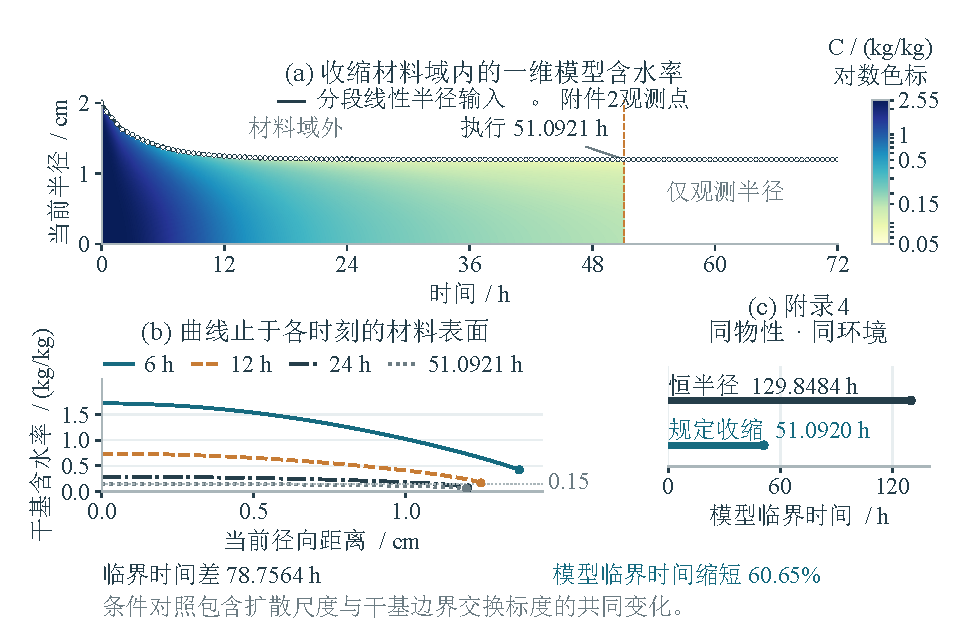
\includegraphics[width=0.92\textwidth]{figures/legibility_process/q4_shrinkage.pdf}
 \caption{规定收缩下的径向有效模型场、观测输入与同物性条件对照。(a)当前实际半径坐标中的含水率色图仅显示至正式执行时刻，采用对数色标；全部观测点及分段线性半径输入保留至72\unit{h}，执行线之后只展示半径。(b)各时刻含水率剖面止于当时材料表面。(c)附录4同物性、同环境下的恒半径与规定收缩临界根对照。临界根与执行时刻分别标示；时间差包含扩散尺度和干基边界交换标度变化。}
 \label{fig:q4-shrinkage}
\end{figure}
\Needspace{3\baselineskip}
图\ref{fig:q4-shrinkage}在当前实际半径坐标中展示规定收缩与含水率演化；上方色图止于正式执行时刻并保留完整半径观测输入，左下剖面止于各时刻的材料表面，右下对照原恒半径与规定收缩的临界时间。
为分离施加收缩历程的作用，另保持附录4和其余条件不变，
将半径固定为2\unit{cm}作受控对照，
临界时间为129.848360839\unit{h}；
施加观测收缩后为51.092003254\unit{h}，
模型临界时间缩短78.7564\unit{h}，约60.6526\%。
这反映当前模型中缩短扩散路径与改变边界交换标度的综合作用。
第三、四问还更换了整套物性，故图\ref{fig:q3-q4-drying}两问约6.382\unit{h}的净差
不能全部归因于收缩。

固定$h_m$保持的是材料干基Robin系数。
在所声明的干质量尺度下，表面质量通量为
$j_s=\rho_d(t)h_m(C_s-b)$，
因而每面积、每单位干基差的通量系数为$K_C=\rho_d h_m$。
当$R/R_0=0.6$时，$K_C$为初始的2.7778倍，
式\eqref{eq:q4-water-ledger}中的$2h_m/R$为初始的1.6667倍。
所以模型临界时间缩短60.6526\%是同一有效方程内的条件对照结果，
不等于固定真实气膜条件下仅由缩短路径得到的效应，也不能据此推断真实热量收支。

\Needspace{3\baselineskip}
半径重建方式也影响终时。
将线性插值改为保形PCHIP，临界时间为$51.088501642\unit{h}$，
比主线提前约12.6058\unit{s}，明显大于单一插值方案内部的数值预算。
输入重建差不能当作半径测量误差的置信区间，适用边界见第\ref{sec:limitations}节。
复现给定的观测$R(t)$不能作为温湿预测的独立验证；改变环境或交换系数而沿用该半径历程时，结果仅为条件响应。

\endgroup
